\chapter{Grundlagen und Begriffsbildung}\label{Kapitel 2}

Es gibt zahlreiche Benchmarks, die bereits an den RPi angepasst und auf diesem ausgef"uhrt wurden. Dabei steht oft die Performance verschiedener Betriebssysteme (z.B. Fedora vs. Debian) oder einzelner Hardware-Komponen\-ten im Vordergrund. Zu diesem Zweck werden haupts"achlich Linux-spezifische Benchmarks verwendet wie Sysbench CPU Benchmark (CPU), PyBench (Python-Implementierung), Apache Benchmark (Webserver), Open\-SSL (CPU) oder ioquake3 (GPU). 

Bei n"aherem Hinschauen erscheint es schwierig, sich einen "Uberblick "uber die existierenden Benchmarks zu verschaffen. Vieles, was von den Anwendern als "`Benchmark"' bezeichnet wird, stellt sich als selbst geschriebene Routine heraus, mit der z.B. die Performance der Grafikkarte getestet werden soll. Eine solche Routine kann f"ur einen Vergleich mit HPC-Rechnern herangezogen werden. Im Folgenden wird daher auf grundlegende Begriffe eingegangen, die f"ur die nachfolgende Untersuchung von Bedeutung sind. Anschlie\ss end werden die verwendeten Benchmarks (vgl. \ref{Benchmarks}) und ihre Anpassung an den RPi erl"autert (vgl. \ref{Aufbau}). 

\section{Definition: Benchmark}\label{Benchmarking}

Unter \textit{Benchmarking} oder "`Ma\ss st"abe vergleichen"' versteht man im Allgemeinen die vergleichende Analyse von Ergebnissen oder Prozessen mit einem festgelegten Bezugswert oder Vergleichsprozess. \textit{Computer-Benchmarks}, die hier von Bedeutung sind, dienen dem Vergleich der Rechenleistung von Computer-Systemen, wozu in der Regel Software verwendet wird\footnote{"`A simple method of measuring performance is by means of a benchmark program. [...] The intention is that by running it upon a new type of machine one may learn something of the performance the machine would have if it ran the original programs \cite{cur76}."'}. Das \textit{Computer Lexikon 2012} kennt folgende Definition: 
\begin{quote}
\onehalfspacing
Mit einem Benchmark-Programm werden Hardwarekomponenten meist auf Geschwindigkeit getestet, wie z.B. die CPU, das Mainboard, die Festplatte (Schreib-Lese-Geschwindigkeit), die Grafikkarte (Frames/s) usw. Verschiedene Benchmark-Programme liefern oft unterschiedliche Ergebnisse, so dass ein direkter Vergleich zwischen den erreichten Werten kaum aussagekr"aftig ist \cite{pre11}. 
\end{quote}
Hieran wird deutlich, dass die Aussagekraft von Benchmarks eng mit der jeweiligen Testumgebung und der Zielsetzung des Benchmarks zusammenh"angt. Zwei Benchmarks, die die CPU-Performance evaluieren, liefern m"oglicherweise unterschiedliche Ergebnisse, weil unterschiedliche Parameter oder sogar Messgr"o\ss en zu Grunde liegen. Das ist insbesondere bei der Auswahl der Implementierungen und Gestaltung der Testumgebung zu ber"ucksichtigen (vgl. Kap. \ref{RPi Spezifikation}, \ref{Spezifikation Bramble} und \ref{Aufbau}). 

In dieser Arbeit soll die Leistung von Hardware-Komponenten eines oder mehrerer parallel arbeitender Rechenkerne mit standardisierten Verfahren ermittelt werden. Rechenberg bezeichnet "`\textit{Analyse}, \textit{Auswahl} und \textit{Konfiguration} von Gesamtsystemen aus Hardware und Software \cite{rec06}"' als eine Hauptaufgabe der Leistungsbewertung: 
\begin{quote}
\onehalfspacing
[F]"ur diese Aufgaben, die die etwa im Zuge einer Rechnerbeschaffung anfallen, wurde in Form von standardisierten Me\ss programmen und -methoden (\textit{benchmarking}) eine solide Basis geschaffen \cite{rec06}. 
\end{quote} 
Daher wird hier hier mit \textit{Benchmarking} kurz das \textbf{\textit{Standardisieren von Arbeit}} bezeichnet.

\section{Definition: Leistung}\label{Leistung}

Die physikalische Gr"o\ss e \textit{Leistung} ist als \textit{Energie pro Zeit} definiert. In der Informatik versteht man darunter meist die \textit{Rechenleistung}. Wichtige Aspekte bei der Leistungsbewertung eines Rechnersystems sind unter anderem
\begin{quote}
\onehalfspacing
[...] die \textit{Leistungskenngr"o\ss en} oder \textit{-ma\ss zahlen} (\textit{performance metrics}), die f"ur das vorliegende Rechnersystem und die Ziele der Leistungsanalyse relevant sind \cite{rec06}.
\end{quote}
Weitere Aspekte der Leistungsbewertung sind das zu untersuchende System, die Workload und die Methode zur Leistungsermittlung\footnote{Vgl. \cite{rec06}.}. "Ubertragen auf die vorliegende Untersuchung bedeutet dies: Das zu untersuchende System besteht aus einem RPi-Einzelrechner und einem RPi-Cluster (vgl. Kap. \ref{RPi Spezifikation} bzw. \ref{Spezifikation Bramble}). Methoden zur Leistungsbewertung sind HPC-Benchmarks (vgl. Kap. \ref{Linpack}, \ref{Whetstone} und \ref{STREAM}). Die Workload ist die Ausf"uhrung dieser Programme. 
Die hier verwendete Definition greift den ersten Aspekt auf: Mit \textit{Leistung} ist die \textbf{\textit{Time to completion}} gemeint, d.h. die Zeit, die ein Prozess oder ein Programm(teil) bis zum erfolgreichen Abschluss ben"otigt. Bei Rechenberg wird dies als "`Programmlaufzeit"' \cite{rec06} bezeichnet\footnote{Andere Klassen von Kenngr"o\ss en, die neben der Zeit zur Leistungsbewertung herangezogen werden, sind \textit{Durchsatz} und \textit{Auslastung}. Abweichende zeitliche Kenngr"o\ss en sind z.B. \textit{Bedienzeit (Service time)} oder \textit{TTR (Time to Response)} (vgl. ebd.).}. 

\section{Definition: Performance}\label{Performance}

F"ur den Begriff \textit{Performance} im Zusammenhang mit Rechnern existieren verschiedene Definitionen, h"aufig gleichbedeutend mit der \textit{Rechenleistung} oder nicht klar davon abgegrenzt. Erkl"arungen wie "`Zeitverhalten von Programmen und Ger"aten"' oder "`Leistungsf"ahigkeit eines Computersystems"' scheinen der Fragestellung nicht ganz gerecht zu werden: 
\begin{quote}
\onehalfspacing
The performance of a computer is a complicated issue, a function of many interrelated quantities. These quantities include the application, the algorithm, the size of a problem, the high-level language, the implementation, the human level of effort used to optimize the program, the compiler's ability to optimize, the age of the compiler, the operating system, the architecture of the computer and the hardware characteristics \cite{don03}.
\end{quote}
Das \textit{Informatik-Handbuch} liefert eine genauere Definition:
\begin{quote} 
\onehalfspacing
Quantitative Leistungsanalysen (\textit{performance analyses}) ermitteln Leistungskenngr"o\ss en von Rechenanlagen. [...] Leistungsbewertung kann sich auf Teilschaltungen, Komponenten (wie Prozessor, Speichersystem oder periphere Ger"ate), gesamte Rechnerverb"unde beziehen \cite{rec06}.
\end{quote}
In dieser Arbeit werden Performance eines RPis und eines RPi-Clusters ermittelt und der Leistungsf"ahigkeit eines Supercomputers gegen"ubergestellt. Der Ma\ss stab f"ur die Performance ist dabei die \textit{Time to Completion} eines gegebenen Benchmark-Programms\footnote{Vgl. hierzu Curnow in Bezug auf Whetstone: "`We are not claiming [to reflect] the overall performance of a given system. On the contrary, we believe that no single number ever can. It does, however, reflect the performance of a dedicated machine for solving a dense system of linear equations \cite{cur76}"'.}. \textit{Performance} soll daher hier als \textbf{\textit{Arbeit pro Zeit}} verstanden werden. 

\section{Benchmarks}\label{Benchmarks}

Aus der F"ulle an existierenden Benchmarks wurden drei f"ur die Untersuchung ausgew"ahlt. Kriterien waren dabei Erprobtheit, Verl"asslichkeit und Angemessenheit f"ur das zu untersuchende System\footnote{Vgl. Weickers Kriterien f"ur die Auswahl eines Benchmarks: "`the [\dots] best benchmark (1) is written in a high-level language, making it portable across different machines, (2) is representative for some kind of programming style (for example, systems programming, numerical programming, or commercial programming), (3) can be measured easily, and (4) has wide distribution \cite{wei90}."'}. Au\ss erdem muss gew"ahrleistet sein, dass der Benchmark "uberhaupt auf das gew"ahlte System anwendbar und an dieses anpassbar ist\footnote{Aus diesem Grund mussten z.B. SHOC und LLNL IOR ausscheiden. SHOC ist nicht lauff"ahig auf dem RPi, da Open CL nicht unterst"utzt wird. LLNL IOR wiederum ben"otigt ein POSIX-, MPIIO- oder HDF5-Interface. Zum letztendlichen Ausschluss von Whetstone vgl. Kap. \ref{Kapitel 5}.}. 

Mit dem Ziel, das Skalierungsverhalten eines RPi-Clusters zu untersuchen, wurden drei etablierte HPC-Benchmarks ausgew"ahlt, die sowohl auf Cluster-Architekturen als auch Einzelrechnern zur Anwendung kommen: Linpack, Whetstone und STREAM. Sie werden im Folgenden vorgestellt. 

\subsection{Linpack}\label{Linpack}

Grunds"atzlich muss man zwischen der Linpack-Library und dem Linpack-Benchmark unterscheiden: Die Library ist eine numerische Programmbibliothek zum L"osen von linearen Gleichungssystemen. Sie wurde inzwischen von anderen Bibliotheken abgel"ost, galt aber lange als Standard\footnote{F"ur die genaue Spezifikation von Linpack vgl. \cite{don03}. Der Sourcecode f"ur Linpack 1000 in Fortran findet sich unter \url{http://www.netlib.org/benchmark/1000d}.}. Der Linpack-Benchmark basiert auf zwei Programmen dieser Bibliothek\footnote{"`Linpack was designed out of a real, purposeful program that is now used as a benchmark\cite{wei90}."'}. Er wurde haupts"achlich von Jack Dongarra, einem der Autoren der Linpack-Bibliothek, entwickelt und wird seit den 1970er Jahren zur Klassifizierung von Rechnern verwendet\footnote{"`Over the years additional performance data was added [...] and today the collection includes over 1300 different computer systems \cite{don03}."'}. Seit 1993 werden die leistungsf"ahigsten Supercomputer der Welt durch die Top500-Rankings ermittelt. Hierzu dient die Variante HPLinpack, auch $N\times N$ Linpack oder High Parallel Computing genannt\footnote{"`Over recent years, the LINPACK Benchmark has evolved from a simple listing for one matrix problem to an expanded benchmark describing the performance at three levels of problem size on several hundred computers. The benchmark today is used by scientists worldwide to evaluate computer performance, particularly for innovative advanced-architecture machines \cite{don03}."' Eine detaillierte Beschreibung des Sourcecode von HPLinpack findet sich ebd..}. 

% MPI: Message Passing Interface

% LU Factorization: 
%Will man das Lösen eines quadratischen eindeutig lösbaren Gleichungssystems Ax=b als Computerprogramm umsetzen, bietet es sich an, den Gaußalgorithmus als LR-Zerlegung (auch LU-Zerlegung oder Dreieckszerlegung genannt) zu interpretieren. Dies ist eine Zerlegung der regulären Matrix A in das Produkt einer linken unteren Dreiecksmatrix L (links, bzw. engl. „lower“) und einer rechten oberen Dreiecksmatrix R (rechts, auch mit U bezeichnet, von engl. „upper“)

% BLAS: Basic Linear Algebra Subroutines

\subsubsection{Funktionsweise}\label{Funktionsweise Linpack}

Linpack ist ein Benchmark zur Ermittlung der CPU-Performance. Dazu werden Flie\ss punkt-Operationen auf einer Matrix\footnote{LINPACK 100: $100 \times 100$-Matrix; LINPACK 1000: $1000\times 1000$-Matrix; HPLinpack: $n\times n$-Matrix (vgl. ebd.).}, die intern in eine lineare Darstellung umgewandelt wird, durchgef"uhrt und das Ergebnis in \textit{FLOPS} ("`Floating Point Operations Per Second"') ausgegeben\footnote{Genau genommen ist es so, dass zwar haupts"achlich, aber nicht ausschlie\ss lich Floating Point-Operationen ausgef"uhrt werden. Der Anteil der Nicht-Flie\ss punkt-Operationen wie Berechnungen auf Integer-Werten werden bei der Auswertung entweder vernachl"assigt oder in die Flie\ss punkt-Operationen integriert (vgl. \cite{wei90}).}. Dabei erreicht der derzeit leistungsf"ahigste Supercomputer, \textit{Tianhe-2 (MilkyWay-2)}, z.B. einen \textit{Rmax}-Wert ("`Maximal LINPACK performance achieved"') von 33862.7 TFLOPS. SuperMUC, der j"ungst auf Platz 10 der Top500 gerankt wurde, erreicht einen Rmax-Wert von 2897.0 TFLOPS.

Beim Vergleich Linpack-Ergebnissen ist die Gr"o\ss e des Arrays bzw. der Matrix von Bedeutung, da eine "Anderung wegen geringerer Datenlokalit"at zu starken Abweichungen der Ergebnisse f"uhren kann\footnote{Vgl. ebd..}. Wichtig ist das beim Vergleich der Ergebnisdaten verschiedener Rechnerarchitekturen. I.d.R. werden daher o.g. standardisierte Gr"o\ss en verwendet, auch wenn der Quellcode eine Ver"anderung der Matrixgr"o\ss e zul"asst. 

\subsubsection{Linpack auf dem Raspberry Pi}\label{Linpack RPi}

Bereits kurz nach Verkaufsstart des RPi wurden Implementierungen von Linpack f"ur den RPi bereit gestellt und Ergebnisse von Testl"aufen im Internet ver"offentlicht\footnote{Die hier verwendete Implementierung in C f"ur den RPi-Einzelrechner findet sich unter \url{http://www.roylongbottom.org.uk/Raspberry_Pi_Benchmarks.zip}.}. Linpack soll als Ausgangspunkt f"ur die Untersuchung dienen, da er sehr gut dokumentiert ist und Vergleichswerte f"ur einen RPi-Einzelrechner bereits vorliegen. Auch Implementierungen von Linpack f"ur verteilte Systeme unabh"angig von den Top500-Rankings sind im Umlauf\footnote{Vgl. \url{http://www.netlib.org/benchmark/hpl/}.}. Zu pr"ufen wird sein, wie diese f"ur den RPi-Cluster nutzbar gemacht werden k"onnen. 

\subsection{Whetstone}\label{Whetstone}

Auch Whetstone ist als Benchmark sowohl im HPC-Bereich als auch zur Klassifizierung von Einzelrechnern seit langen Jahren etabliert\footnote{"`[\dots] the most common 'stone age' benchmarks (CPU/memory/compiler benchmarks only) [are] in particular the Whetstone, Dhrystone, and Linpack benchmarks. These are the benchmarks whose results are most often cited in manufacturers' publications and in the trade press \cite{wei90}."'}. Er wurde 1976 von Roy Longbottom u.A. entwickelt und gilt als erstes Programm, das jemals explizit f"ur das Benchmarking industrieller Standards designt wurde\footnote{Vgl. ebd..}. Wie Linpack misst er die CPU-Performance. 

\subsubsection{Funktionsweise}\label{Funktionsweise Whetstone}

Die Funktionsweise von Whetstone "ahnelt Linpack. Allerdings werden nicht nur Flie\ss komma-Berechnungen ausgef"uhrt, sondern auch mathematische Funktionen, Integer-Arithmetik, If-Statements etc. kommen zur Anwendung\footnote{Ein Grund hierf"ur ist, dass die urspr"ungliche Programmversion nicht komplex genug war, um ein durchschnittliches FORTRAN-Programm zu simulieren. Gegen"uber der urspr"unglichen Implementierung in ALGOL 60 war ein damals "ublicher FORTRAN-Compiler in der Lage, Zwischenergebnisse in schnellen Registern abzuspeichern und darauf zur"uckzugreifen, sodass die gemessene CPU-Leistung deutlich h"oher ausfiel als erwartet (vgl. \cite{cur76}).}. Jedes dieser als genuin betrachteten Module wird in eine For-Schleife eingebettet und viele Male  hintereinander ausgef"uhrt. Die Ausgabe der Berechnungsergebnisse ist Teil des Programms\footnote{Allerdings: "`This output is only required to ensure that the calculations are logically necessary; it is not intended to represent the output from a typical program"' (ebd.).}. Ein Framework bildet den "au\ss eren Programmrahmen und steuert die Ausgaben der einzelnen Module. Die Ergebnisse wurden zun"achst in \textit{Whetstone Instructions per Second} gemessen, heutige Implementierungen liefern Ergebnisse in MFLOPS\footnote{F"ur eine detaillierte Darstellung der Entwicklung und Implementierung von Whetstone vgl. ebd.. Hier findet sich auch der urspr"ungliche Sourcecode in ALGOL 60.}. 

% Least-squares: 
%Die Methode der kleinsten Quadrate ist das mathematische Standardverfahren zur Ausgleichungsrechnung. Dabei wird zu einer Datenpunktwolke eine Kurve gesucht, die möglichst nahe an den Datenpunkten verläuft.

\subsubsection{Whetstone auf dem Raspberry Pi}\label{Whetstone RPi}

Whetstone erschien wie f"ur den RPi gemacht, da er sich als Standard f"ur Mini-Computer etabliert hat\footnote{Ein Grund hierf"ur ist, dass Whetstone in den 70er Jahren f"ur Maschinen mit signifikant geringerer Rechenleistung entwickelt worden war. Auch damals gingen die Entwickler von notwendigen Anpassungen f"ur neue Speicherhierarchien aus: "`When more is known about the characteristics of programs running on these multi-level store machines it may be possible to produce a typical program for particular types of machine. [...] Despite these limitations the program described should be of some value, particularly in relation to smaller machines (ebd.)."'}. Er wurde vom Entwickler selbst f"ur den RPi adaptiert und auf diesem getestet\footnote{Vgl. \url{http://www.roylongbottom.org.uk/Raspberry\%20Pi\%20Benchmarks.htm}.}. Auch hier liegen also bereits Vergleichswerte f"ur einen RPi-Einzelrechner vor. 

Wie f"ur die meisten etablierten HPC-Benchmarks existieren Implementierungen in zahlreichen h"oheren Programmiersprachen wie C, C++, Fortran und Java\footnote{Vgl. z.B. \url{http://freespace.virgin.net/roy.longbottom/}.}. Auch hier wird aus nahe liegenden Gr"unden auf eine Implementierung in C f"ur den RPi-Einzelrechner zur"uckgegriffen\footnote{Der hier verwendete Sourcecode findet sich ebenfalls unter \url{http://www.roylongbottom.org.uk/Raspberry_Pi_Benchmarks.zip}.}. Ob eine lauff"ahige Implementierung f"ur die Cluster-Architektur existiert, wird sich zeigen m"ussen. 
% TODO 
\section{STREAM}\label{STREAM}
% TODO 
\subsection{Funktionsweise STREAM}\label{Funktionsweise STREAM}
% TODO 
\subsection{STREAM auf dem Raspberry Pi}\label{STREAM RPi}
% TODO 
\section{Spezifikation des Raspberry Pi Modell B}\label{RPi Spezifikation}

Was dem Nutzer zuerst auff"allt, ist sicherlich die Gr"o\ss e des RPi. Er wird manchmal als "`Scheckkarten-Computer"' bezeichnet und "uberschreitet diese Ma\ss e mit 85.60 mm $\times$ 53.98 mm $\times$ 17 mm tats"achlich nur geringf"ugig. 
\begin{figure}[htb]
	\centering
	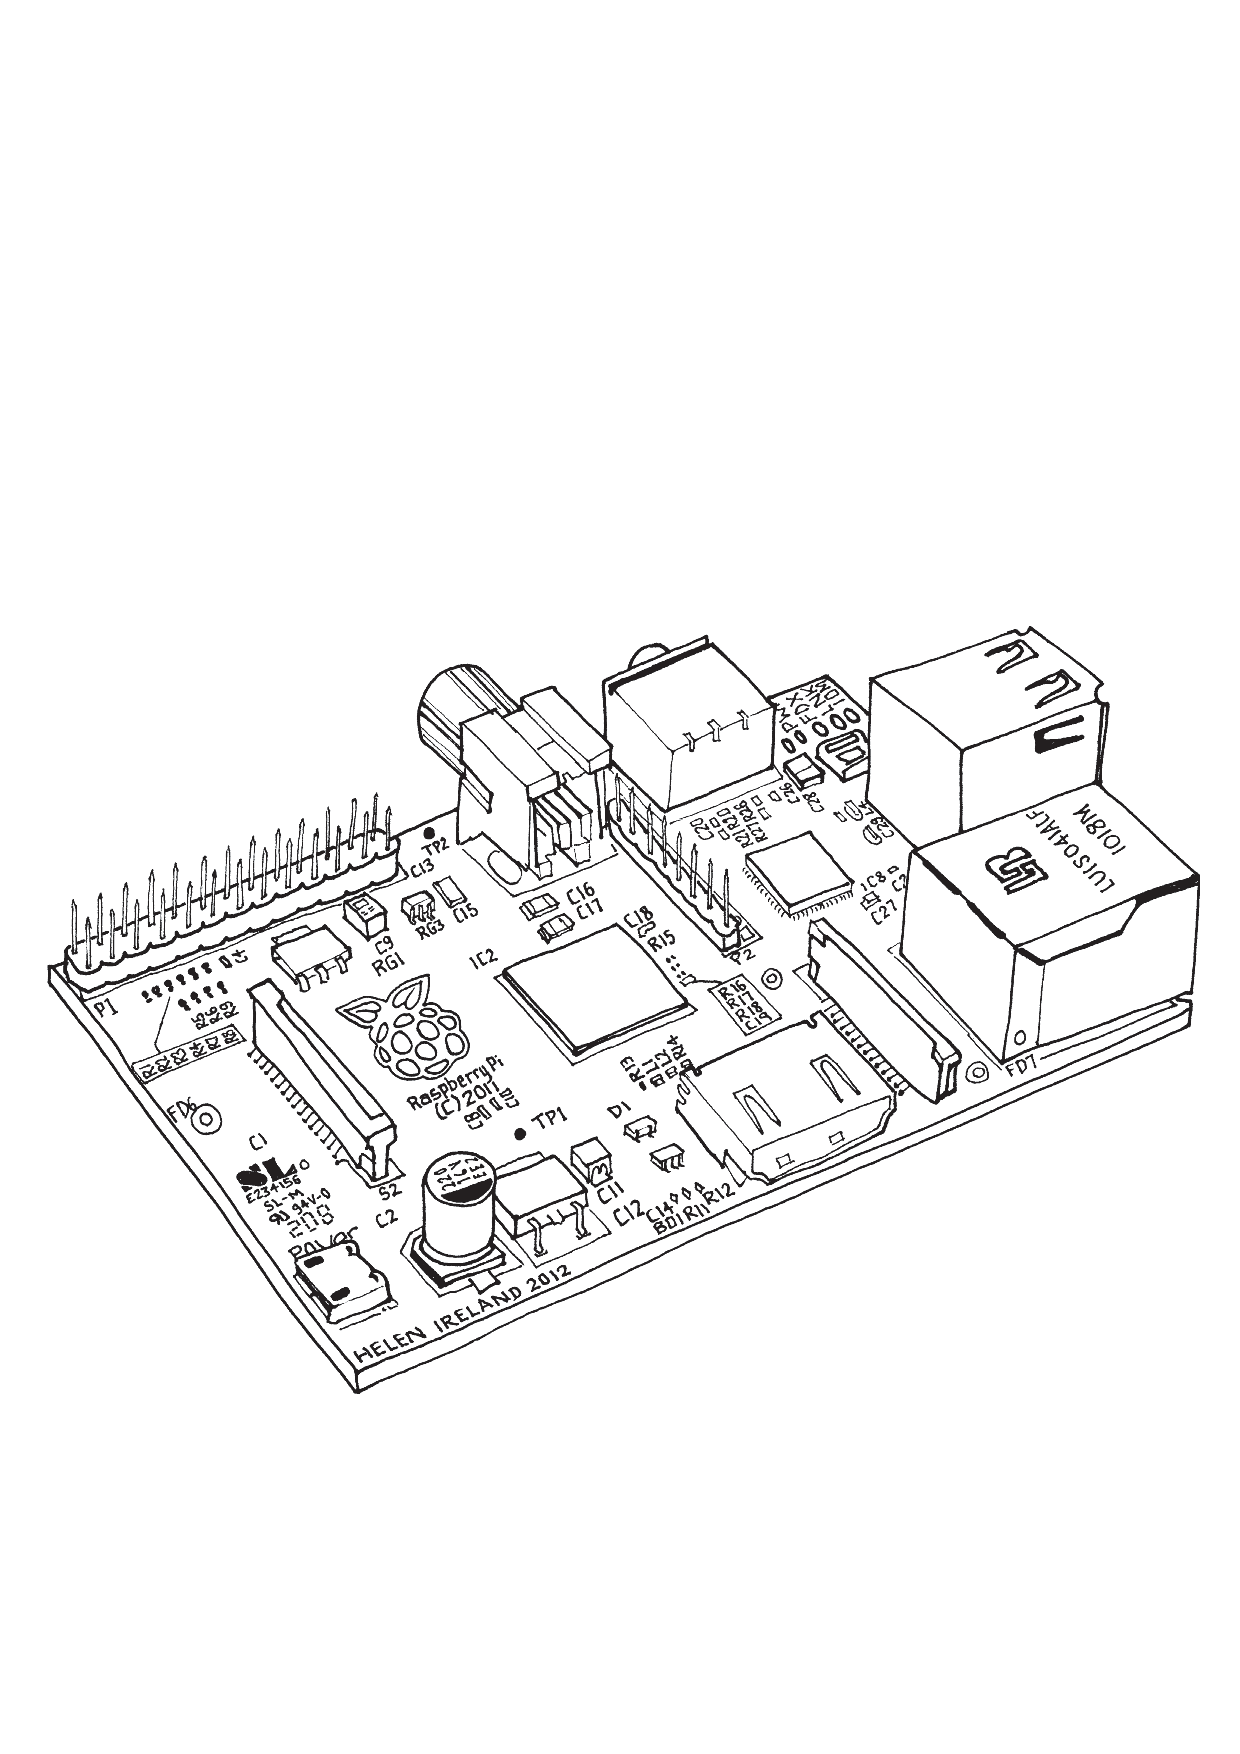
\includegraphics[width=0.7\textwidth]{rpi_grafik.pdf}\\ 
	\caption{Ein Raspberry Pi Modell B\cite{scrguide01}.}\label{fig:RPi-Spezifikation}
\end{figure}

\noindent Auf dieser Platine sind alle Komponenten verbaut, die den RPi zu einem voll funktionsf"ahigen Rechner machen: 

\subsection{SoC, CPU und GPU}\label{RPi Hardware}

Der RPi ist mit einem Broadcom BCM2835 als SoC ausgestattet. Es enth"alt CPU (ein ARM1176JZFS-Prozessor) und GPU (ein Broadcom VideoCore IV-Koprozessor)\footnote{Vgl. \cite{scrguide02}.}. Auff"allig ist, dass die CPU des RPi (ein ARM-Chip, wie er h"aufig in Mobiltelefonen verbaut ist), relativ schwach ist im Vergleich zur GPU, die Full HD-Aufl"osung und das hardwarebeschleunigte Rendern verschiedener Videoformate unterst"utzt. 

\subsection{Arbeitsspeicher}\label{RPi RAM}
Das Modell B des RPi verf"ugt "uber 512 MB SDRAM (gegen"uber dem Modell A mit 256 MB)\footnote{Vgl. ebd..}. Dieser kann nicht erweitert werden. Allerdings teilen sich CPU und GPU den Arbeitsspeicher und diese Einteilung kann durchaus ver"andert werden. Da der RPi kein BIOS hat, ist die Manipulation der Datei \verb+/boot/start.elf+ die einzige M"oglichkeit, RAM zu allokieren\footnote{Vgl. \cite{pow12}.}.

\subsection{Ausg"ange, Hauptspeicher und Stromversorgung}\label{RPi Schnittstellen}

Der RPi verf"ugt "uber einen HDMI-Ausgang, einen Cinch-Ausgang ("`RCA Jack"') und einen analogen Tonausgang. Er hat zwei USB 2.0-Schnittstellen und eine Ethernet-Schnittstelle. Ein Steckplatz ist f"ur eine SD-Karte vorgesehen, auf der der nicht fl"uchtige Speicher liegt. Die Stromversorgung erfolgt "uber einen Mini-USB-Eingang. Zum Betrieb werden mindestens 700 mA/5 V ben"otigt\footnote{Vgl. \cite{pow12}.}. 

\subsection{GPIO/CSI}\label{RPi GPIO} 

Der RPi hat eine GPIO mit 6 Anschl"ussen, die jeweils "uber 26 Pins verf"ugen. "Uber die GPIOs k"onnen LEDs, Sensoren, Displays und andere Ger"ate angesteuert werden. I.d.R. wird dazu der GPIO-Connector P1 verwendet. Zur Steuerung der GPIOs existieren Bibliotheken f"ur verschiedene Programmiersprachen wie C, C++ und Python. Sie k"onnen auch "uber ein Terminal oder Web-Interfaces wie WebIOPi angesprochen werden. 

Von den vorhandenen Ein- und Ausg"angen werden beim Versuchsaufbau lediglich Ethernet, Mini-USB und der Steckplatz f"ur die Speicherkarte verwendet. Beim RPi-Einzelrechner erfolgt der Netzanschluss "uber einen DSL-Router, wodurch der RPi ins interne Heimnetz eingebunden wird. Beim RPi-Cluster erfolgen Stromversorgung und Netzanschluss zentral "uber den Server des RPi-Clusters. Jeder RPi-Node verf"ugt "uber eine eigene Speicherkarte. Auf die Cluster-Architektur wird in Kap. \ref{Spezifikation Bramble} genauer eingegangen\footnote{Eine detaillierte Beschreibung findet sich in \cite{kli13}}

\subsection{Betriebssystem}\label{RPi OS}

F"ur den RPi existieren mehrere Implementierungen bzw. Derivate verbreiteter Betriebssysteme, darunter RISC OS und Plan 9. Am verbreitetsten sind Linux/Unix-basierte Systeme wie FreeBSD und NetBSD (BSD-Varianten), Raspbian (Debian-Variante), Pidora (Fedora-Variante) oder eine Variante von Arch Linux\footnote{Vgl. ebd..}.   

\section{Raspberry Pi-Cluster als Testumfeld}\label{Spezifikation Bramble}

In den letzten Monaten zeigte sich verst"arkt die Tendenz, eine gr"o\ss ere Anzahl von Raspberry Pis zu einem Cluster zu koppeln\footnote{Weitere Cluster-Projekte werden z.B. in \cite{cox13}, \cite{kie01}, \cite{bal12} und \cite{ou13} dargestellt.}. Im Folgenden wird die hier verwendete Architektur kurz vorgestellt\footnote{F"ur eine detaillierte Beschreibung vgl. \cite{kli13}.}. 

\subsection{Aufbau}\label{Bramble Hardware}
Der RPi-Cluster besteht aus 20 RPi Modell B-Einzelrechnern, die jeweils mit einem Ethernet-Kabel mit einem zentralen x86-Server (bestehend haupts"achlich aus einem Mini-ITX-Mainboard und einer Gigabit Ethernet-Netzwerkkarte) verbunden sind. Sie befinden sich in einem modifizierten Tower-Metallgeh"ause, das auf die Seite gedreht und oben offen gelassen wurde. Darin sind au\ss erdem ein 24 Port Gigabit-Switch, die Stromversorgung des Servers und der RPis sowie die K"uhlung integriert\footnote{Ein solches System relativ kosteng"unstiger Rechnermit einem BSD- oder Linux-Betriebssystem, die "uber IP kommunizieren, wird im Allgemeinen als \textit{Beowulf} bezeichnet (vgl. \cite{kie01} und \cite{kli13}). H"aufig dient es dem Ersatz oder der Simulation eines Supercomputers. Im Zusammenhang mit RPis ist auch der Begriff \textit{Bramble} gebr"auchlich, der im Folgenden verwendet wird (vgl. \url{www.raspberrypi.org/archives/tag/bramble}).}. 
% TODO Cluster fotografieren und Bild einbinden 
\begin{figure}[htb]
	\centering
	\includegraphics[width=0.7\textwidth]{bramble.pdf}\\ 
	\caption{Der hier verwendete Bramble.}\label{fig:Bramble}
\end{figure}

% NIC = Network Interface Card 

\subsection{Betriebssystem und Filesystem}\label{Bramble Systemarchitektur} 

Wie in Kap. \ref{RPi OS} beschrieben, existieren verschiedene Linux-Varianten f"ur den RPi. Als Betriebssytem f"ur den RPi-Einzelrechner und die Bramble-RPis wurde Raspbian, die offizielle Distribution der Raspberry Pi Foundation, gew"ahlt\footnote{Vgl. \url{http://www.raspberrypi.org/faqs}. Das verwendete Image findet sich unter \url{http://downloads.raspberrypi.org/raspbian_latest}.}. Auf den Einsatz von NOOBS\footnote{Die Raspberry Pi-Foundation empfiehlt besonders f"ur Einsteiger die \textit{New Out Of Box Software} und bietet entsprechend pr"aparierte SD-Karten zum Kauf an (vgl. \url{http://www.raspberrypi.org/archives/tag/noobs}).} oder anderer zus"atzlicher Bootloader wurde verzichtet\footnote{In diesem Fall fungiert die ausf"uhrbare Datei \texttt{start.elf}, die nach einer ausf"uhrbaren Datei \texttt{kernel.img} sucht und diese l"adt, als Bootloader (vgl. \cite{kli13}).}. Auf dem Server selbst l"auft eine Standard-Debian-Version. 

Ein Charakteristikum eines Beowulf-Clusters bzw. Bramble ist, dass es im Gegensatz zu einem "`richtigen"' Supercomputer kein Shared Memory-Interface und keine Cache-Koh"arenz gibt. Die Kommunikation zwischen den einzelnen Komponenten via Ethernet ist zudem relativ langsam. Es stellt sich daher die Frage nach dem Filesystem und der Synchronisierung der einzelnen Nodes. 

Um das Filesystem der einzelnen Nodes mit dem NFS des Servers zu synchronisieren, wurde hier eine Read-Only-Schicht f"ur die Slaves (Nodes) und eine Read-Write-Schicht f"ur den Master (Server) verwendet\footnote{Vgl. ebd..}. Um trotzdem die M"oglichkeit des gemeinsamen Zugriffs der Nodes auf ein Speichermedium zu haben, wurde ein geshartes Verzeichnis \texttt{/srv} eingerichtet. 

\subsection{Zugriff}\label{Bramble Zugriff}

Welche M"oglichkeiten gibt es nun, verteilte Anwendungen auf dem Bramble auszuf"uhren bzw. "uberhaupt die einzelnen Komponenten anzusprechen? Bei einem RPi-Einzelrechner nutzt man normalerweise einen USB-Port und den HDMI-Ausgang als stdin bzw. stdout. Eine andere M"oglichkeit besteht darin, den RPi "uber den Ethernet-Port mit einem Router zu verbinden und via SSH aus dem Intranet darauf zuzugreifen\footnote{Auf dem hier verwendeten Testger"at wurde letztere Variante gew"ahlt. Der Grund hierf"ur sind bekannte Probleme beim Anschluss "alterer Monitore oder Fernseher ohne HDMI-Eingang (vgl. z.B. \url{http://www.raspberrypi.org/forum/viewtopic.php?f=91&t=34061}).}. 

Der Zugriff auf den Bramble erfolgt ebenfalls aus dem internen Netzwerk via IP und SSH. Da sich die Architekturen des Servers und der RPi-Nodes unterscheiden, ist die einzige M"oglichkeit, auf diese zuzugreifen, wiederum via IP und SSH. Es gibt auf jedem RPi den Raspbian-Standard-User \texttt{pi}, der hier nicht ver"andert wurde\footnote{Auf dem RPi-Einzelrechner wurden aus Sicherheitsgr"unden Username und Passwort f"ur den Standard-User ge"andert.}. Um z.B. auf das gesharte Verzeichnis \texttt{/srv} zuzugreifen, sind \texttt{root}-Rechte erforderlich. 
\endinput 
